\documentclass{beamer}
\usepackage{relsize}
\usepackage{color}

\usepackage{listings}
\usetheme{CambridgeUS}
%\usepackage{beamerthemesplit} % new 
\usepackage{enumitem}
\usepackage{amsmath}                    % See geometry.pdf to learn the layout options. 
\usepackage{amsthm}                   % See geometry.pdf to learn the layout options. There 
\usepackage{amssymb}                    % See geometry.pdf to learn the layout options. 
\usepackage[utf8]{inputenc} 
\usepackage{graphicx}
\usepackage[english,bulgarian]{babel}

\lstset{language=C++,
                basicstyle=\ttfamily,
                keywordstyle=\color{blue}\ttfamily,
                stringstyle=\color{red}\ttfamily,
                commentstyle=\color{green}\ttfamily,
                morecomment=[l][\color{magenta}]{\#}
}

\newtheorem{mydef}{Дефиниция}[section]
\newtheorem{lem}{Лема}[section]
\newtheorem{thm}{Твърдение}[section]

\DeclareMathOperator{\restrict}{\upharpoonright}

\setitemize{label=\usebeamerfont*{itemize item}%
  \usebeamercolor[fg]{itemize item}
  \usebeamertemplate{itemize item}}

\setbeamercovered{transparent}



\begin{document}
\title[Увод в програмирането]{Изчислителен процес. Блок схеми. Състояние на програмата. Блокове в C++. Начални сведения за масиви и символни низове} 
\author{Калин Георгиев} 
\frame{\titlepage} 


\section{Литература} 



\begin{frame}[fragile]
\frametitle{Препоръчителна литература}

\relscale{0.9}

\textbf{Основна}

\begin{itemize}

\item М. Тодорова. Програмиране на C++ - първа част, С. СИЕЛА , 2002.
\item М. Тодорова, П. Армянов, Д. Зотева, К. Георгиев. Сборник от задачи по програмиране на C++. Част първа. Увод в програмирането, ТехноЛогика ЕООД, 2008.

\end{itemize}


\textbf{Допълнителна}


\begin{itemize}

\item  Niklaus Wirth,  Algorithms + Data Structures = Programs, Prentice-Hall Series in Automatic Computation 
\item Robert Sedgewick, Algorithms in C++
\item П. Наков, П. Добриков, Програмиране = ++Алгоритми; С., Top Team Co, 2003.
Допълнителна:
\item Л. Амерал, Алгоритми и структури от данни в C++, С, СОФТЕХ, 2001.
\item Липман, Езикът C++ в примери, С., КОЛХИДА ТРЕИД – КООП, 1993.

\end{itemize}


\end{frame}



\section{Изчислителен процес} 


\begin{frame}
\centerline{Изчислителен процес}
\end{frame}

\begin{frame}[fragile]
\frametitle{Последоватленост на операциите и ``състояние''}


\begin{columns}[c]
  \begin{column}{0.3\textwidth}
\begin{lstlisting}
int a,b;
\end{lstlisting}

  \end{column}
  \begin{column}{0.7\textwidth}
\begin{tabular}{ c | c | c | c}
\hline
... & a & b &  ...\\\hline
... & ? & ? & ... \\\hline
  
\end{tabular}

  \end{column}
\end{columns}

\pause

\begin{columns}[c]
  \begin{column}{0.3\textwidth}
\begin{lstlisting}
a = 5;
\end{lstlisting}

  \end{column}
  \begin{column}{0.7\textwidth}
\begin{tabular}{ c | c | c | c}
\hline
... & a & b &  ...\\\hline
... & \alert{5} & ? & ... \\\hline
  
\end{tabular}

  \end{column}
\end{columns}

\pause

\begin{columns}[c]
  \begin{column}{0.3\textwidth}
\begin{lstlisting}
b = 10;
\end{lstlisting}

  \end{column}
  \begin{column}{0.7\textwidth}
\begin{tabular}{ c | c | c | c}
\hline
... & a & b &  ...\\\hline
... & 5 & \alert{10} & ... \\\hline
  
\end{tabular}

  \end{column}
\end{columns}

\pause

\begin{columns}[c]
  \begin{column}{0.3\textwidth}
\begin{lstlisting}
b = a + b;
\end{lstlisting}

  \end{column}
  \begin{column}{0.7\textwidth}
\begin{tabular}{ c | c | c | c}
\hline
... & a & b &  ...\\\hline
... & 5 & \alert{15} & ... \\\hline
  
\end{tabular}

  \end{column}
\end{columns}

\pause

\begin{columns}[c]
  \begin{column}{0.3\textwidth}
\begin{lstlisting}
b = a + b;
\end{lstlisting}

  \end{column}
  \begin{column}{0.7\textwidth}
\begin{tabular}{ c | c | c | c}
\hline
... & a & b &  ...\\\hline
... & 5 & \alert{20} & ... \\\hline
  
\end{tabular}

  \end{column}
\end{columns}

\end{frame}


\begin{frame}
\centerline{Блок схеми и процеси}
\end{frame}


\begin{frame}[fragile]
\frametitle{Линейна програма}

%X\vspace*{800pt}
\hspace*{-30pt}
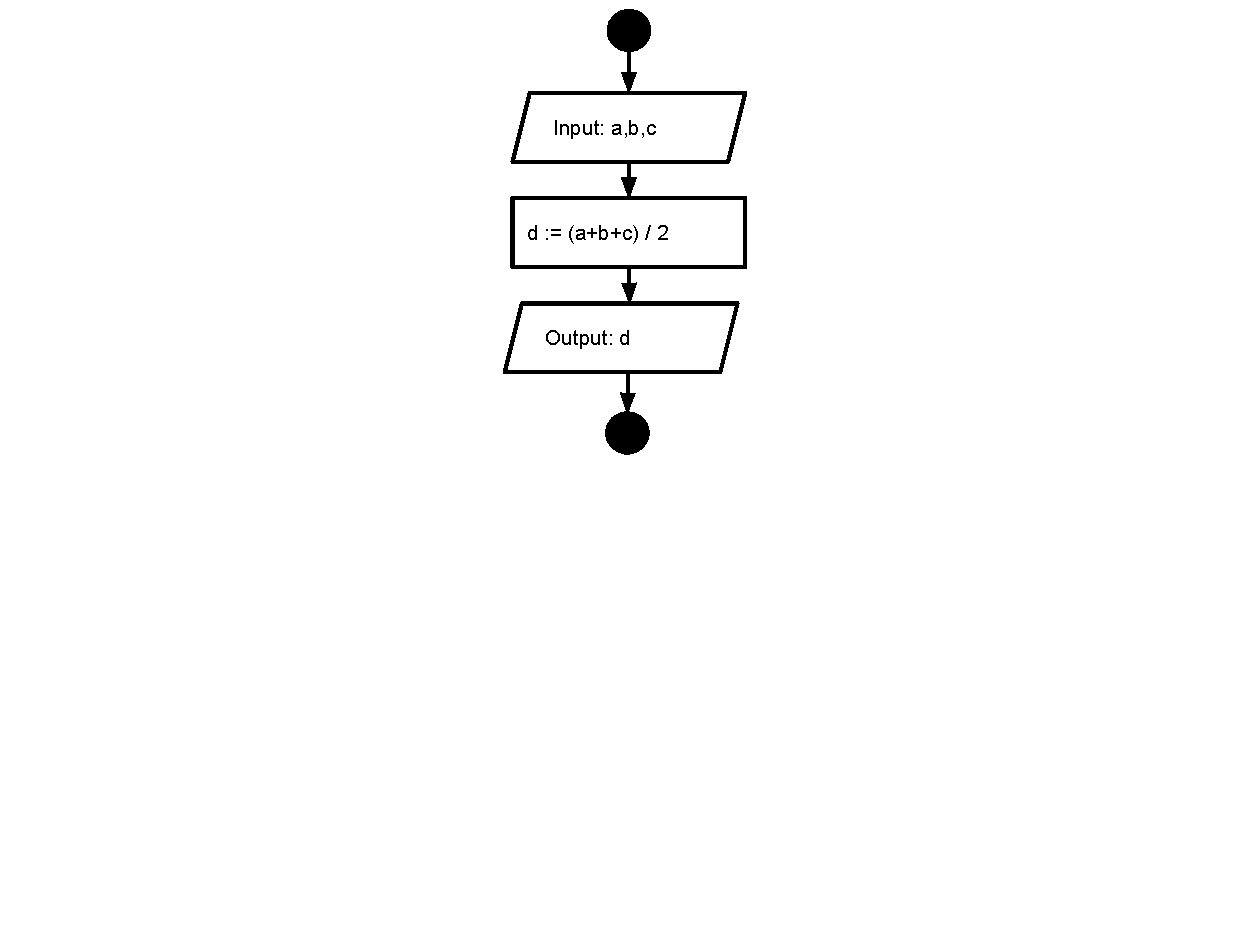
\includegraphics[width=14cm]{images/fc_linear} 

\end{frame}


\begin{frame}[fragile]
\frametitle{Линейна програма}

%X\vspace*{800pt}
\hspace*{-30pt}
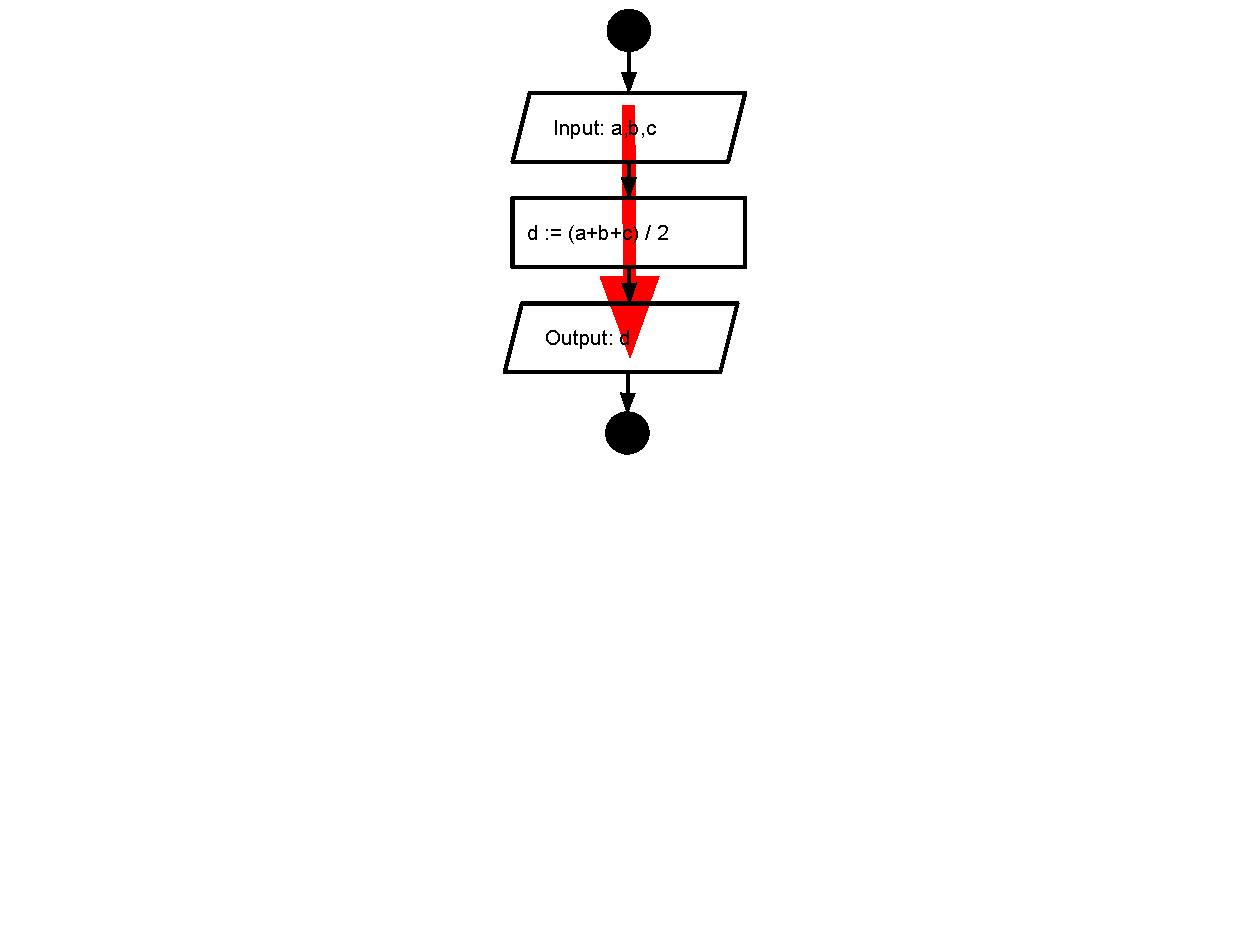
\includegraphics[width=14cm]{images/fc_linear_arrows} 

\end{frame}


\begin{frame}[fragile]
\frametitle{Разклонение}

%X\vspace*{800pt}
\hspace*{-30pt}
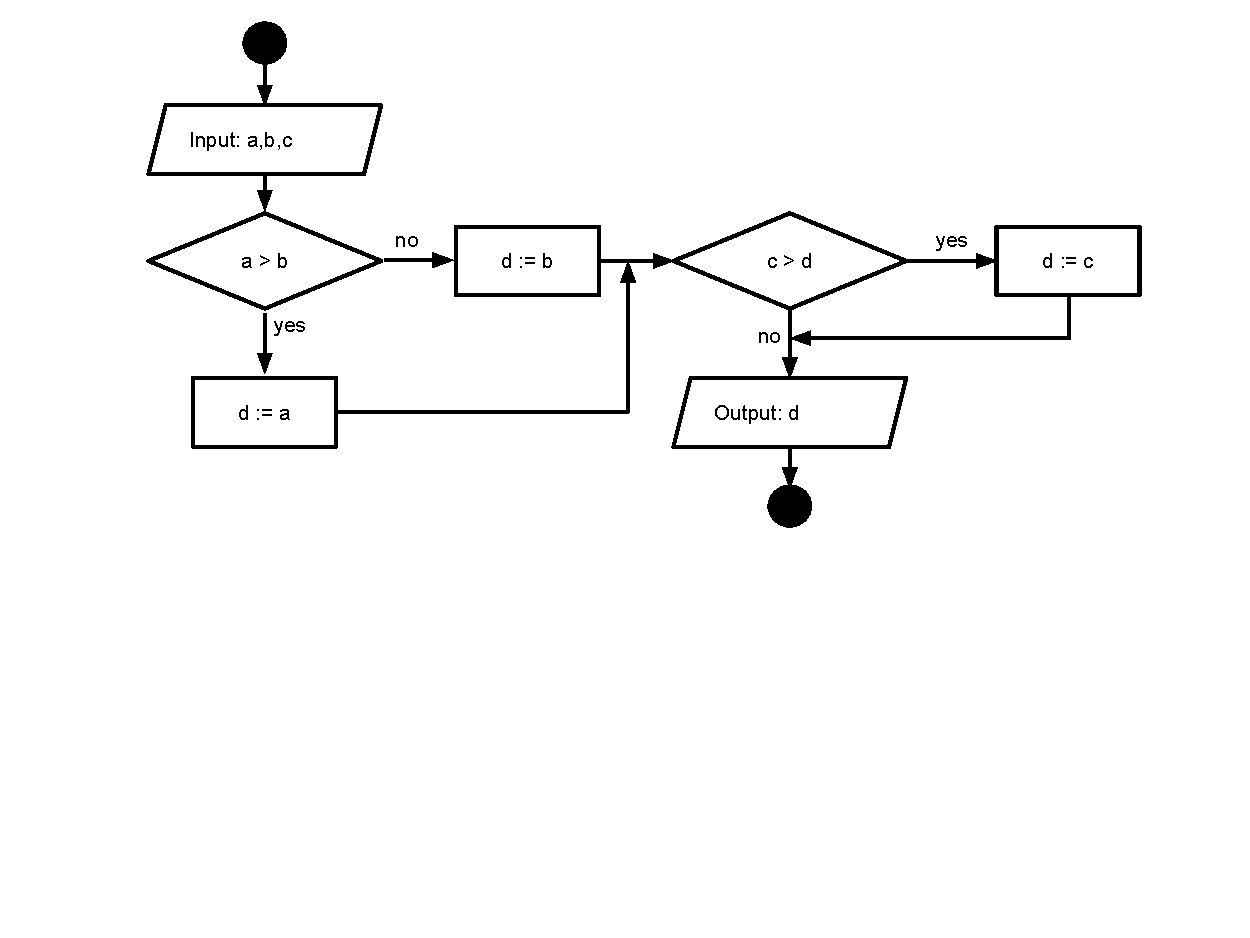
\includegraphics[width=14cm]{images/fc_if} 

\end{frame}


\begin{frame}[fragile]
\frametitle{Разклонение}

%X\vspace*{800pt}
\hspace*{-30pt}
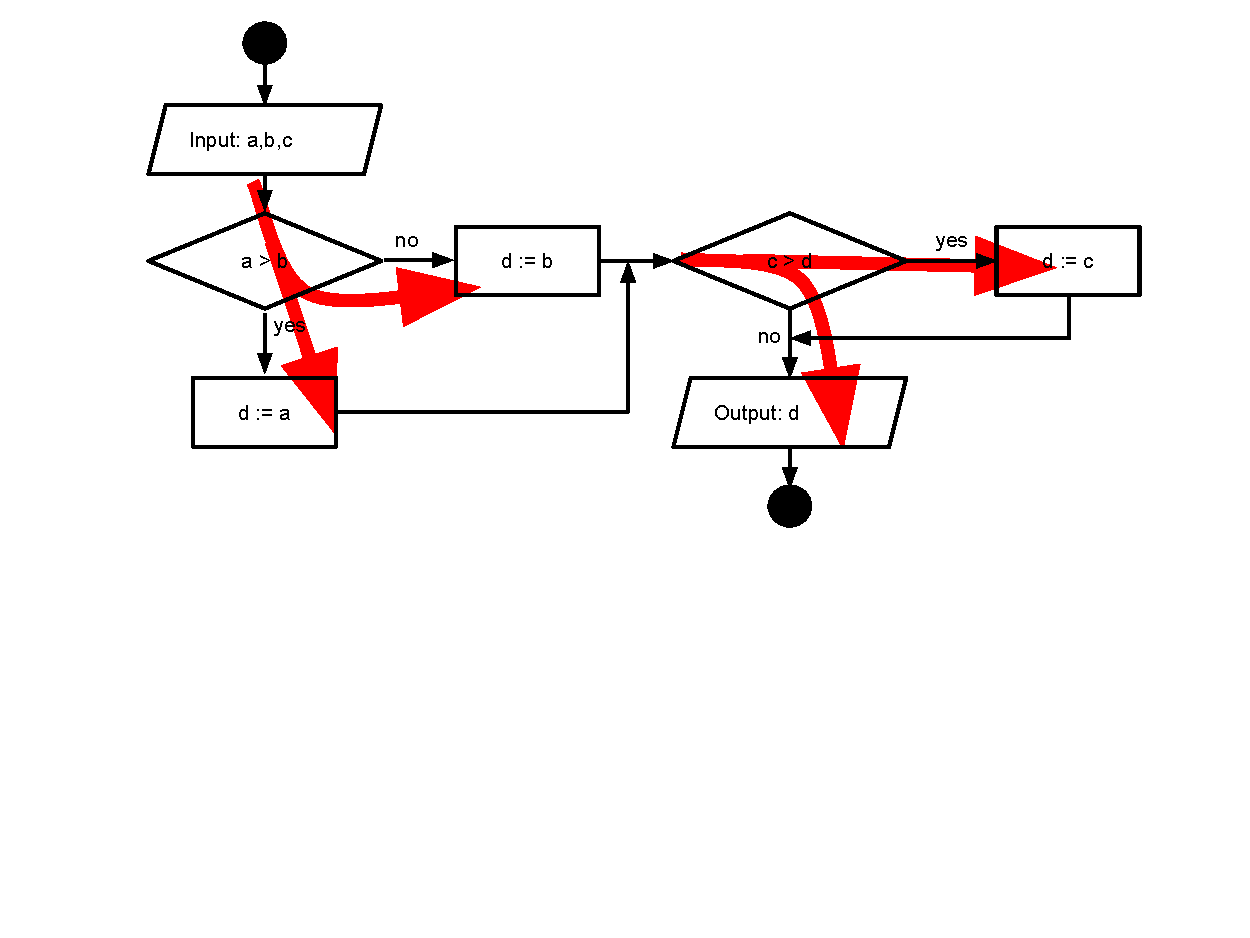
\includegraphics[width=14cm]{images/fc_if_arrows} 

\end{frame}

\begin{frame}[fragile]
\frametitle{Цикъл}

%X\vspace*{800pt}
\hspace*{-30pt}
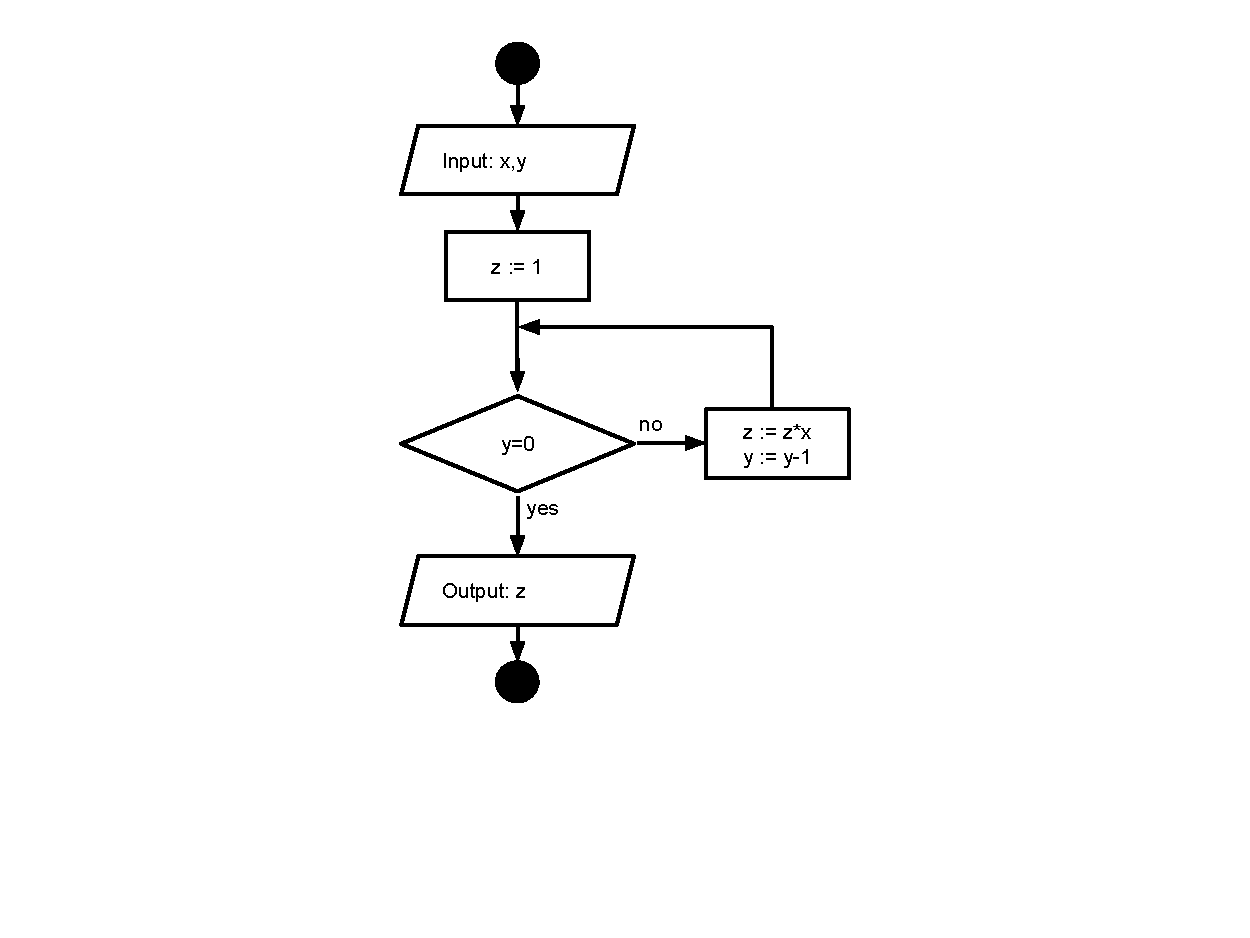
\includegraphics[width=14cm]{images/fc_cycle} 

\end{frame}


\begin{frame}[fragile]
\frametitle{Цикъл}

%X\vspace*{800pt}
\hspace*{-30pt}
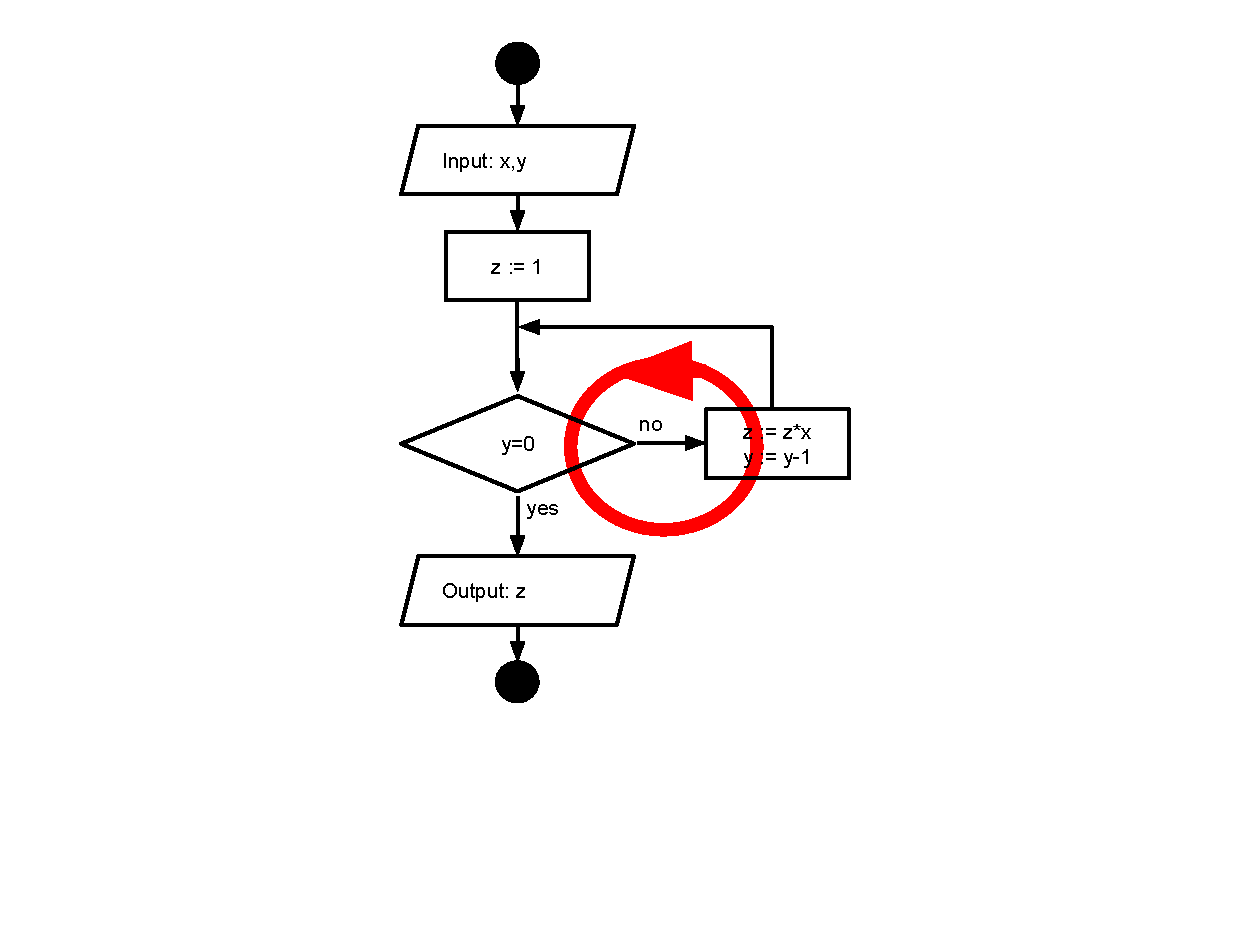
\includegraphics[width=14cm]{images/fc_cycle_arrows} 

\end{frame}



\begin{frame}[fragile]
\frametitle{$x^y$}


\begin{columns}[c]
  \begin{column}{0.3\textwidth}
\begin{tabular}{ c | c | c | c  }
\hline
\# & x & y & z \\\hline
0 & 2 & 5 & 1 \\\hline
1 & 2 & 4 & 2 \\\hline
2 & 2 & 3 & 4 \\\hline
3 & 2 & 2 & 8 \\\hline
4 & 2 & 1 & 16 \\\hline
5 & 2 & 0 & 32 \\\hline
  
\end{tabular}

  \end{column}
  \begin{column}{0.7\textwidth}

%X\vspace*{800pt}
\hspace*{-90pt}
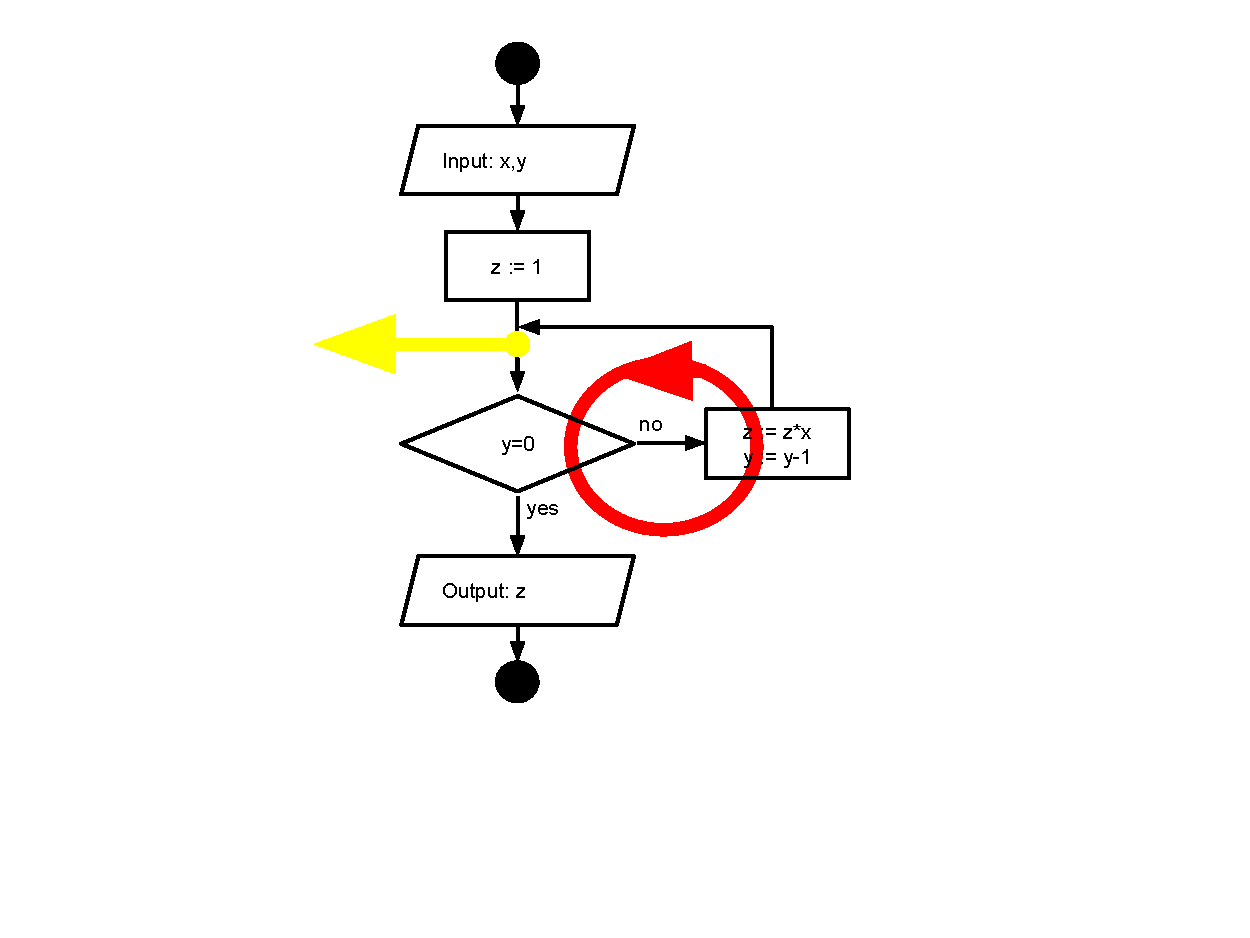
\includegraphics[width=12cm]{images/fc_cycle_arrows_2} 


  \end{column}
\end{columns}


\end{frame}

\section{While} 


\begin{frame}
\centerline{Още един вид цикъл в C++}
\end{frame}


\begin{frame}[fragile]
\frametitle{Неструктурирани езици}

\begin{columns}[t]
  \begin{column}{0.3\textwidth}
\relscale{0.7}

\begin{verbatim}
10. Въведи X и Y
20. Z := 1
30. Ако Y == 0 GOTO 70
40. Z := Z * X
50. Y := Y -1
60. GOTO 30
70. Отпечатай Z
80. Край   
\end{verbatim}

  \end{column}
  \begin{column}{0.7\textwidth}

%X\vspace*{800pt}
\hspace*{-90pt}
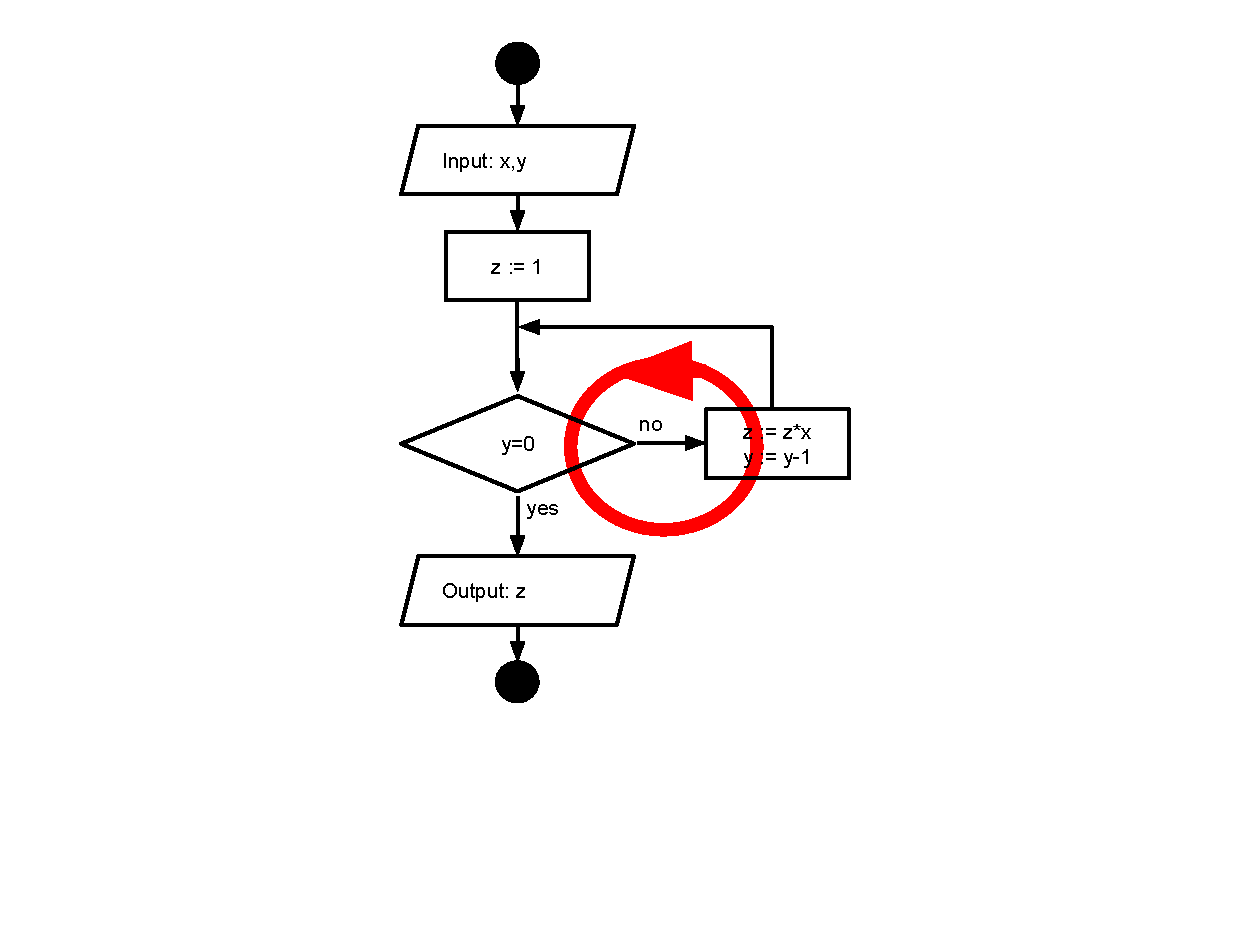
\includegraphics[width=12cm]{images/fc_cycle_arrows} 


  \end{column}
\end{columns}


\end{frame}


\begin{frame}[fragile]
\frametitle{Цикъл While}


\begin{columns}[t]
  \begin{column}{0.3\textwidth}
\relscale{0.7}
\begin{lstlisting}
int x,y,z;

cin >> x >> y;

z = 1;

while (y != 0)
{
  z = z * x;
  y--;
}

cout << y;

\end{lstlisting}

  \end{column}
  \begin{column}{0.7\textwidth}

%X\vspace*{800pt}
\hspace*{-90pt}
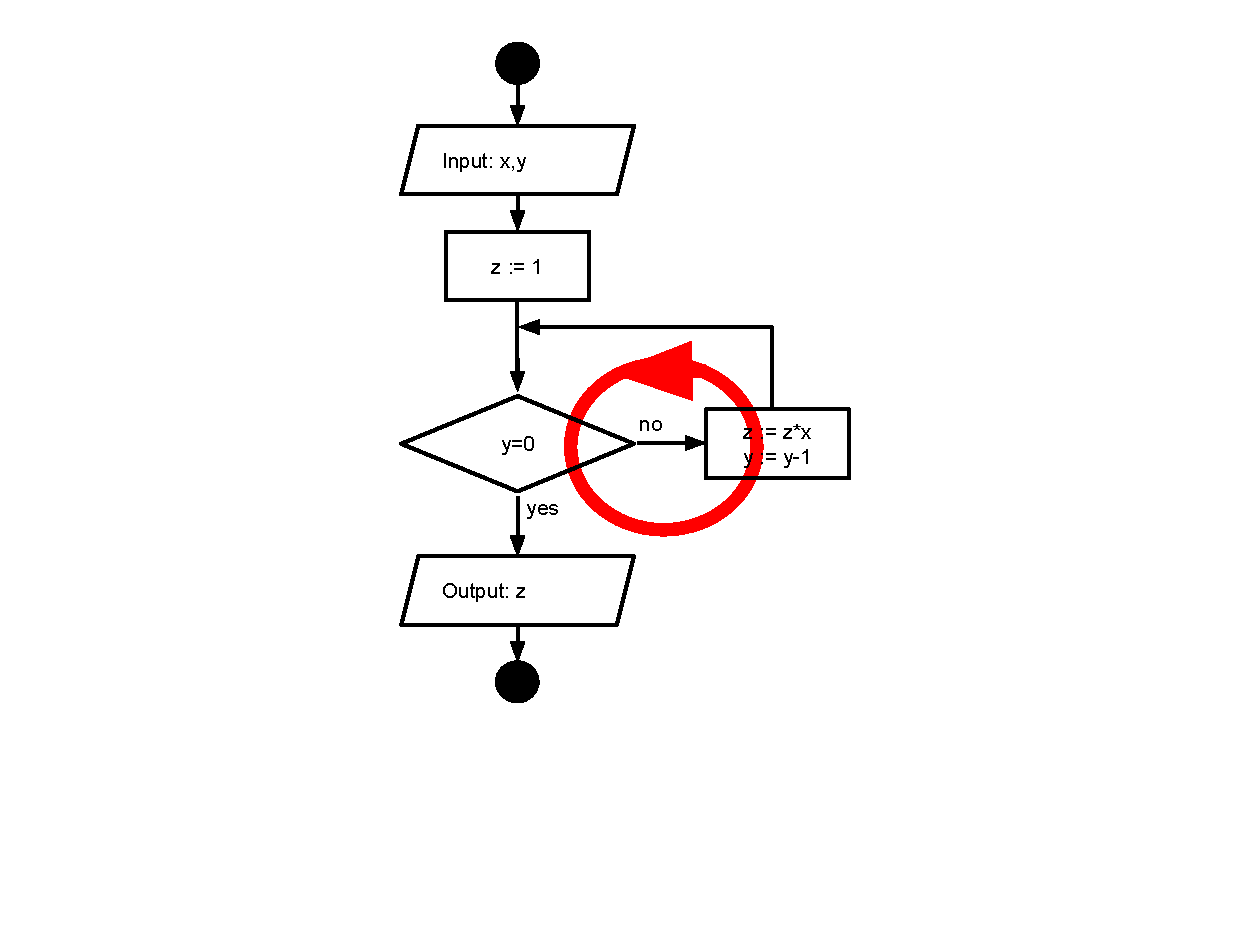
\includegraphics[width=12cm]{images/fc_cycle_arrows} 


  \end{column}
\end{columns}


\end{frame}


\begin{frame}[fragile]
\frametitle{Сравнение}


\begin{columns}[t]
  \begin{column}{0.25\textwidth}
\relscale{0.7}
\begin{lstlisting}
int x,y,z;

cin >> x >> y;

z = 1;

while (y != 0)
{
  z = z * x;
  y--;
}

cout << y;

\end{lstlisting}


  \end{column}
  \begin{column}{0.25\textwidth}

\relscale{0.7}

\begin{verbatim}
10. Въведи X и Y
20. Z := 1
30. Ако Y == 0 GOTO 70
40. Z := Z * X
50. Y := Y -1
60. GOTO 30
70. Отпечатай Z
80. Край   
\end{verbatim}

  \end{column}
  \begin{column}{0.5\textwidth}

%X\vspace*{800pt}
\hspace*{-70pt}
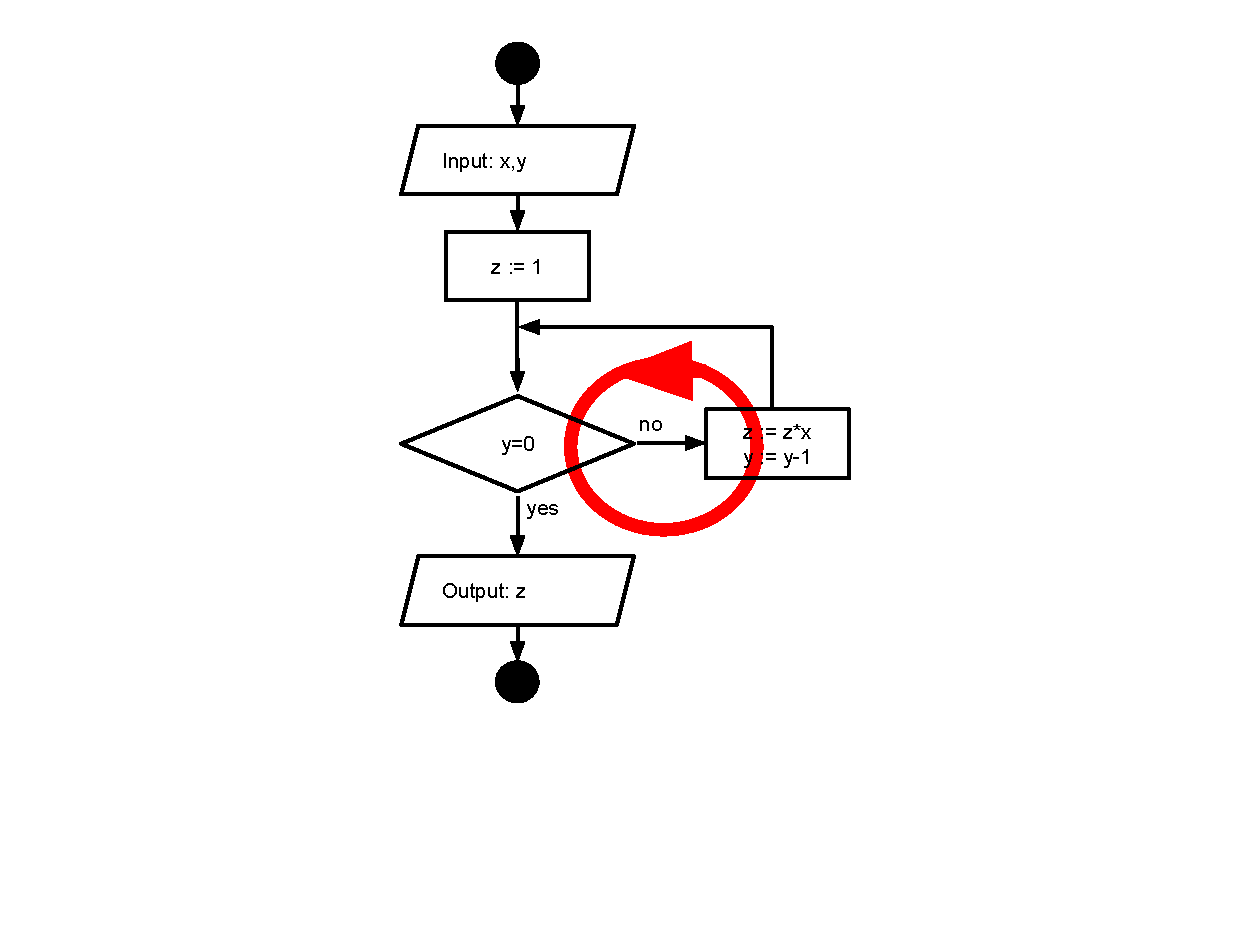
\includegraphics[width=11cm]{images/fc_cycle_arrows} 


  \end{column}
\end{columns}


\end{frame}


\begin{frame}[fragile]
\frametitle{Примери}

\begin{itemize}
  \item Намиране на броя на цифрите в десетичния запис на естествено число
  \item $n!$
  \item Намиране на сумата на цифрите в десетичния запис на естествено число
  \item Проверка дали дадено естествено число притежава цифрата 5 в десетичния си запис
\end{itemize}

\end{frame}


\section{Блокове} 


\begin{frame}
\centerline{Блокове в C++}
\end{frame}


\begin{frame}[fragile]
\frametitle{Какво е блок?}

\begin{lstlisting}
int a = 0;

int b = a + 10;

if (a == 0)
{
  int b = a;
  cout << b;
  b = 100;
}

cout << b;

\end{lstlisting}



\end{frame}


\begin{frame}[fragile]
\frametitle{Стек от променливи}


\begin{columns}[c]
  \begin{column}{0.3\textwidth}
\begin{lstlisting}
int a = 0;
int b = a + 10;
\end{lstlisting}

  \end{column}
  \begin{column}{0.7\textwidth}
\begin{tabular}{ c | c | c | c}
\hline
... & a & b &  ...\\\hline
... & 0 & 10 & ... \\\hline
  
\end{tabular}

  \end{column}
\end{columns}

\pause

\begin{columns}[c]
  \begin{column}{0.3\textwidth}
\begin{lstlisting}
if (a == 0)
{
  int b = a;
  cout << b;
\end{lstlisting}

  \end{column}
  \begin{column}{0.7\textwidth}
\begin{tabular}{ c | c | c | c | c}
\hline
... & a & b &  \alert{b} & ...\\\hline
... & 0 & 10 & \alert {0} & ... \\\hline
  
\end{tabular}

  \end{column}
\end{columns}

\pause

\begin{columns}[c]
  \begin{column}{0.3\textwidth}
\begin{lstlisting}
  b = 100;
\end{lstlisting}

  \end{column}
  \begin{column}{0.7\textwidth}
\begin{tabular}{ c | c | c | c | c}
\hline
... & a & b & b &  ...\\\hline
... & 5 & 10& \alert{100} & ... \\\hline
  
\end{tabular}

  \end{column}
\end{columns}

\pause

\begin{columns}[c]
  \begin{column}{0.3\textwidth}
\begin{lstlisting}
}
\end{lstlisting}

  \end{column}
  \begin{column}{0.7\textwidth}
\begin{tabular}{ c | c | c | c | c}
\hline
... & a & b & \alert{X} &  ...\\\hline
... & 0 & 10 & \alert{X} &... \\\hline
  
\end{tabular}

  \end{column}
\end{columns}

\pause

\begin{columns}[c]
  \begin{column}{0.3\textwidth}
\begin{lstlisting}
cout << b;
\end{lstlisting}

  \end{column}
  \begin{column}{0.7\textwidth}
\begin{tabular}{ c | c | c | c}
\hline
... & a & b &  ...\\\hline
... & 0 & 10 & ... \\\hline
  
\end{tabular}

  \end{column}
\end{columns}

\end{frame}




\section{Масиви и низове} 

\begin{frame}
\centerline{Първоначални сведения за масиви и низове}
\end{frame}

\begin{frame}[fragile]
\frametitle{Представяне на низове}

\begin{itemize}
  \item ASCii таблица 
\end{itemize}

\begin{tabular}{c | c | c | c | c}
\hline
...&$A^{65}$&$B^{66}$&$C^{67}$&... \\\hline
  
\end{tabular}

\pause

\begin{itemize}
  \item Представяне в паметта 
\end{itemize}

\begin{tabular}{c | c | c | c | c | c | c | c}
\hline
...&H &E &L &L &O & \_ &... \\\hline
...&72&69&76&76&79& 0 &... \\\hline
\end{tabular}

\pause
\begin{itemize}
  \item Масиви
\end{itemize}


\end{frame}

\begin{frame}[fragile]
\frametitle{Масиви}

\begin{itemize}
  \item Дефиниране чрез тип и размер: 

\begin{lstlisting}
int arr[100];
\end{lstlisting}
\pause
  \item Достъп до всеки отделен елемент:

\begin{lstlisting}
int b = arr[18];
cin >> arr[18];
b = arr[1] + arr[2];
\end{lstlisting}
\pause

  \item Обхождане с for цикъл

\begin{lstlisting}
for (int count = 0; count < 100; count++)
{
  cout << arr[count];
}
\end{lstlisting}
\end{itemize}

\end{frame}


\begin{frame}[fragile]
\frametitle{Прост пример с низове}

\begin{flushleft}
\relscale{0.5}
\begin{lstlisting}
int main ()
{

  char str[100] = "Hello world!";
  cout << str << endl;

  str[0] = 'Y';
  cout << str << endl;

  cout << "Please input a string:";
  cin >> str;

  for (int counter = 0; counter < 100; counter++)
  {
    if (str[counter] == 'a')
    {
      str[counter] = 'b';
    }
  }

  cout << str << endl;

  return 0;
}
\end{lstlisting}
\end{flushleft}

\end{frame}


\begin{frame}[fragile]
\frametitle{Какво не можем да праивм с масиви и низове}

\begin{itemize}
  \item Няма проверка за коректност!
\end{itemize}

\begin{flushleft}
\relscale{0.75}
\begin{lstlisting}
char a[6] = "HELLO";
a[10] = '!';
\end{lstlisting}


\begin{tabular}{c | c | c | c | c | c | c | c | c | c}
\hline
...&0 &1 &2 &3 &4 &5   &...&10&... \\\hline
...&H &E &L &L &O & \_ &...&\alert{!}& ... \\\hline
\end{tabular}
\end{flushleft}

\pause

\begin{itemize}
  \item Присвояване (a=b)
  \pause
  \item Сравнение (a==b, a < b,...)
\end{itemize}

\end{frame}


\begin{frame}[fragile]
\frametitle{Вградени функции за работа с низове}

\begin{columns}[t]

  \begin{column}{0.6\textwidth}
\relscale{0.5}
  \textbf{Дължина на низ}
\begin{lstlisting}
cout << strlen(a);
\end{lstlisting}
  \textbf{Присвояване на низове}
\begin{lstlisting}
strcpy (d,a);
strcpy (c,a); //!!!
\end{lstlisting}
  \textbf{Сравнение на низове}
\begin{lstlisting}
if (strcmp (a,b) < 0) 
  {cout << "a<b";} 
else 
  {cout << "b<=a";};
\end{lstlisting}
  \textbf{Конкатенация на низове}
\begin{lstlisting}
strcpy (d,a); //d -> "HELLO"
\end{lstlisting}


\begin{tabular}{c | c | c | c | c | c | c | c | c | c | c | c | c }
\hline
...&0 &1 &2 &3 &4 &5 &6 &7 &8 &9 &10   &... \\\hline
...&H &E &L &L &O &\_ &? &? &? &? &? &... \\\hline
\end{tabular}

\begin{lstlisting}
strcat (d,b); //d -> "HELLOWORLD"
\end{lstlisting}

\begin{tabular}{c | c | c | c | c | c | c | c | c | c | c | c | c }
\hline
...&0 &1 &2 &3 &4 &5 &6 &7 &8 &9 &10   &... \\\hline
...&H &E &L &L &O &W &O &R &L &D &\_ &... \\\hline
\end{tabular}



  \end{column}


  \begin{column}{0.4\textwidth}

\begin{flushleft}
\relscale{0.5}
\begin{lstlisting}
#include <cstring>
...
char a[6] = "HELLO";
char b[6] = "WORLD";
char c[4] = "BYE";
char d[11] = "???";
\end{lstlisting}

\begin{tabular}{c | c | c | c | c | c | c | c }
\hline
...&0 &1 &2 &3 &4 &5   &... \\\hline
...&H &E &L &L &O & \_ &... \\\hline
\end{tabular}

\begin{tabular}{c | c | c | c | c | c | c | c }
\hline
...&0 &1 &2 &3 &4 &5   &... \\\hline
...&W  &O &R &L &D & \_ &... \\\hline
\end{tabular}

\begin{tabular}{c | c | c | c | c | c  }
\hline
...&0 &1 &2 &3   &... \\\hline
...&B &Y &E & \_ &... \\\hline
\end{tabular}

\end{flushleft}

  \end{column}
\end{columns}


\end{frame}

\end{document}


\begin{columns}[t]
  \begin{column}{0.2\textwidth}

  \end{column}
  \begin{column}{0.8\textwidth}

  \end{column}
\end{columns}


